\documentclass[a0paper,portrait]{baposter}

\usepackage{wrapfig}
\usepackage{lmodern}

\usepackage{graphicx} 
\usepackage{subfig}
\usepackage{bm}
\usepackage{amsmath}
\usepackage{mathtools} % Provides \prescript command

\usepackage[utf8]{inputenc} %unicode support
\usepackage[T1]{fontenc}
\usepackage{gensymb} %°


\selectcolormodel{cmyk}

\graphicspath{{figures/}} % Directory in which figures are stored
\renewcommand{\figurename}{Fig.} %rename figure

\newcommand{\compresslist}{%
\setlength{\itemsep}{0pt}%
\setlength{\parskip}{1pt}%
\setlength{\parsep}{0pt}%
}

\newenvironment{boenumerate}
  {\begin{enumerate}\renewcommand\labelenumi{\textbf\theenumi.}}
  {\end{enumerate}}

  \let\oldthebibliography\thebibliography
  \let\endoldthebibliography\endthebibliography
  \renewenvironment{thebibliography}[1]{
    \begin{oldthebibliography}{#1}
      \setlength{\itemsep}{0em}
      \setlength{\parskip}{0em}
  }
  {
    \end{oldthebibliography}
  }

\begin{document}

\definecolor{PUC}{cmyk}{0.58,0.34,0,0.29}

\begin{poster}
{
grid=false,
headerborder=closed, % Adds a border around the header of content boxes
colspacing=1em, % Column spacing
bgColorOne=white, % Background color for the gradient on the left side of the poster
bgColorTwo=white, % Background color for the gradient on the right side of the poster
borderColor=PUC, % Border color
headerColorOne=PUC, % Background color for the header in the content boxes (left side)
headerColorTwo=PUC, % Background color for the header in the content boxes (right side)
headerFontColor=white, % Text color for the header text in the content boxes
boxColorOne=white, % Background color of the content boxes
textborder=rectangle, %rectangle, % Format of the border around content boxes, can be: none, bars, coils, triangles, rectangle, rounded, roundedsmall, roundedright or faded
eyecatcher=true, % Set to false for ignoring the left logo in the title and move the title left
headerheight=0.135\textheight, % Height of the header
headershape=rectangle, % Specify the rounded corner in the content box headers, can be: rectangle, small-rounded, roundedright, roundedleft or rounded
headershade=plain,
headerfont=\Large\textsf, % Large, bold and sans serif font in the headers of content boxes
%textfont={\setlength{\parindent}{1.5em}}, % Uncomment for paragraph indentation
linewidth=2pt % Width of the border lines around content boxes
}
%
%----------------------------------------------------------------------------------------
%	TITLE AND AUTHOR NAME
%----------------------------------------------------------------------------------------
%
{ %eyecatcher

\includegraphics[scale=0.2]{figures/LogoAndes.jpeg}
}
{ % Poster title
\textsf{\Huge Thorium Fuel Cycle in Nuclear Reactors}
}
{% Author names
\sf\huge\vspace{0.3em}
F. Garcia  \& J. Sanabria.\\
\vspace{0.1em}
\small{
Departamento de física, Universidad de los Andes, Bogotá, Colombia. \\
\vspace{0.1em}
fw.garcia@uniandes.edu.co}
}


\headerbox{Abstract}{name=Abstract,column=0,row=0, span=3}{
  This project explores the potential of thorium-based nuclear fuels in Pressurized Water Reactors (PWRs), focusing on the thorium fuel cycle and its various implementations. The research investigates the benefits and challenges associated with thorium fuel, including its higher conversion ratios, improved thermal properties, and intrinsic proliferation resistance. Detailed simulations using OpenMC analyze the behavior of thorium oxide (ThOX) with \(\prescript{233}{}{U}\) at different concentrations. The results demonstrate that while thorium-based fuels can achieve breeding, maintaining criticality presents challenges. The project also examines the impact of fuel composition and concentration on reactor performance and safety. The findings suggest that optimizing these parameters is crucial for enhancing the performance and safety of thorium-based fuels. The research concludes with a discussion on the future prospects of thorium in the nuclear industry and the need for further research and development to fully realize its potential as a sustainable nuclear fuel.
}




\headerbox{1. Introduction}{name=Introduction, span=1,column=0,below=Abstract}{
  At the time, there were concerns that the global supply of \(\prescript{235}{}{U}\) would be insufficient to meet future energy demands. Weinberg and his colleagues recognized that molten salt reactors (MSRs) could be used to breed \(\prescript{233}{}{U}\) from thorium \cite{TMSR_book}. Between 1965 and 1969, ORNL successfully operated an MSR experiment for 15 months, achieving an impressive \(87\%\) operational uptime, even utilizing \(\prescript{233}{}{U}\) as fuel \cite{TMSR_book}. Despite this success, the MSR program was eventually discontinued as other nuclear concepts received greater political support \cite{IAEA2005}. Thorium is not a fissile material but rather a fertile material, so the idea of the thorium fuel cycle is to breed \(\prescript{233}{}{U}\).

  \begin{center}
    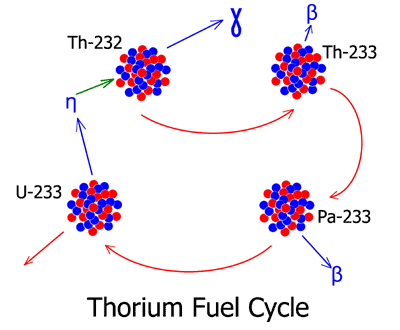
\includegraphics[scale=0.25]{Th_breeding.png}
    \captionof{figure}{\footnotesize \(\prescript{233}{}{U}\) breeding from \(\prescript{232}{}{Th}\). Image retrive from \textbf{Ref.} \cite{Donev2024}}
  \end{center}
}


\headerbox{2. Simulations}{name=Simulations, span=1,column=0,below=Introduction}{
  The simulation uses OpenMC, a Monte Carlo neutron transport simulation library developed by the Computational Reactor Physics Group (CRPG) at MIT. The objective was to analyze the behavior of thorium-based nuclear fuels in a PWR as a reference for other reactor types. In this project, a Pressurized Water Reactor (PWR) simulation was conducted to evaluate different thorium fuel cycles.

  \begin{center}
  
\includegraphics[scale=0.16]{OpenMC_logo.png}
  \captionof{figure}{\footnotesize OpenMC Logo. Image retrive from \textbf{Ref.} \cite{OpenMC}.}
  \end{center}

}


\headerbox{3. Results}{name=Results, span=2,column=1,below= Abstract}{
  Simulations were conducted using uranium oxide fuel with thorium concentrations of \(10\%\) and \(50\%\). The results indicated that increasing the thorium concentration improved the conversion ratio, consistent with findings in \cite{N_Improvement}. However, higher thorium concentrations also presented challenges in maintaining criticality. The results suggest that while higher thorium concentrations can enhance fuel utilization, careful optimization of fuel composition and reactor parameters is essential to ensure stable and efficient reactor operation. \textbf{Fig.} \ref{fig:Th_10} shows the isotopes concentration in the fuel as a function of time for a \(10\%\) thorium concentration. Additional, \textbf{Fig.} \ref{fig:Th_10_r} shows the reactivity as a function of time for the same thorium concentration.

  \begin{center}
    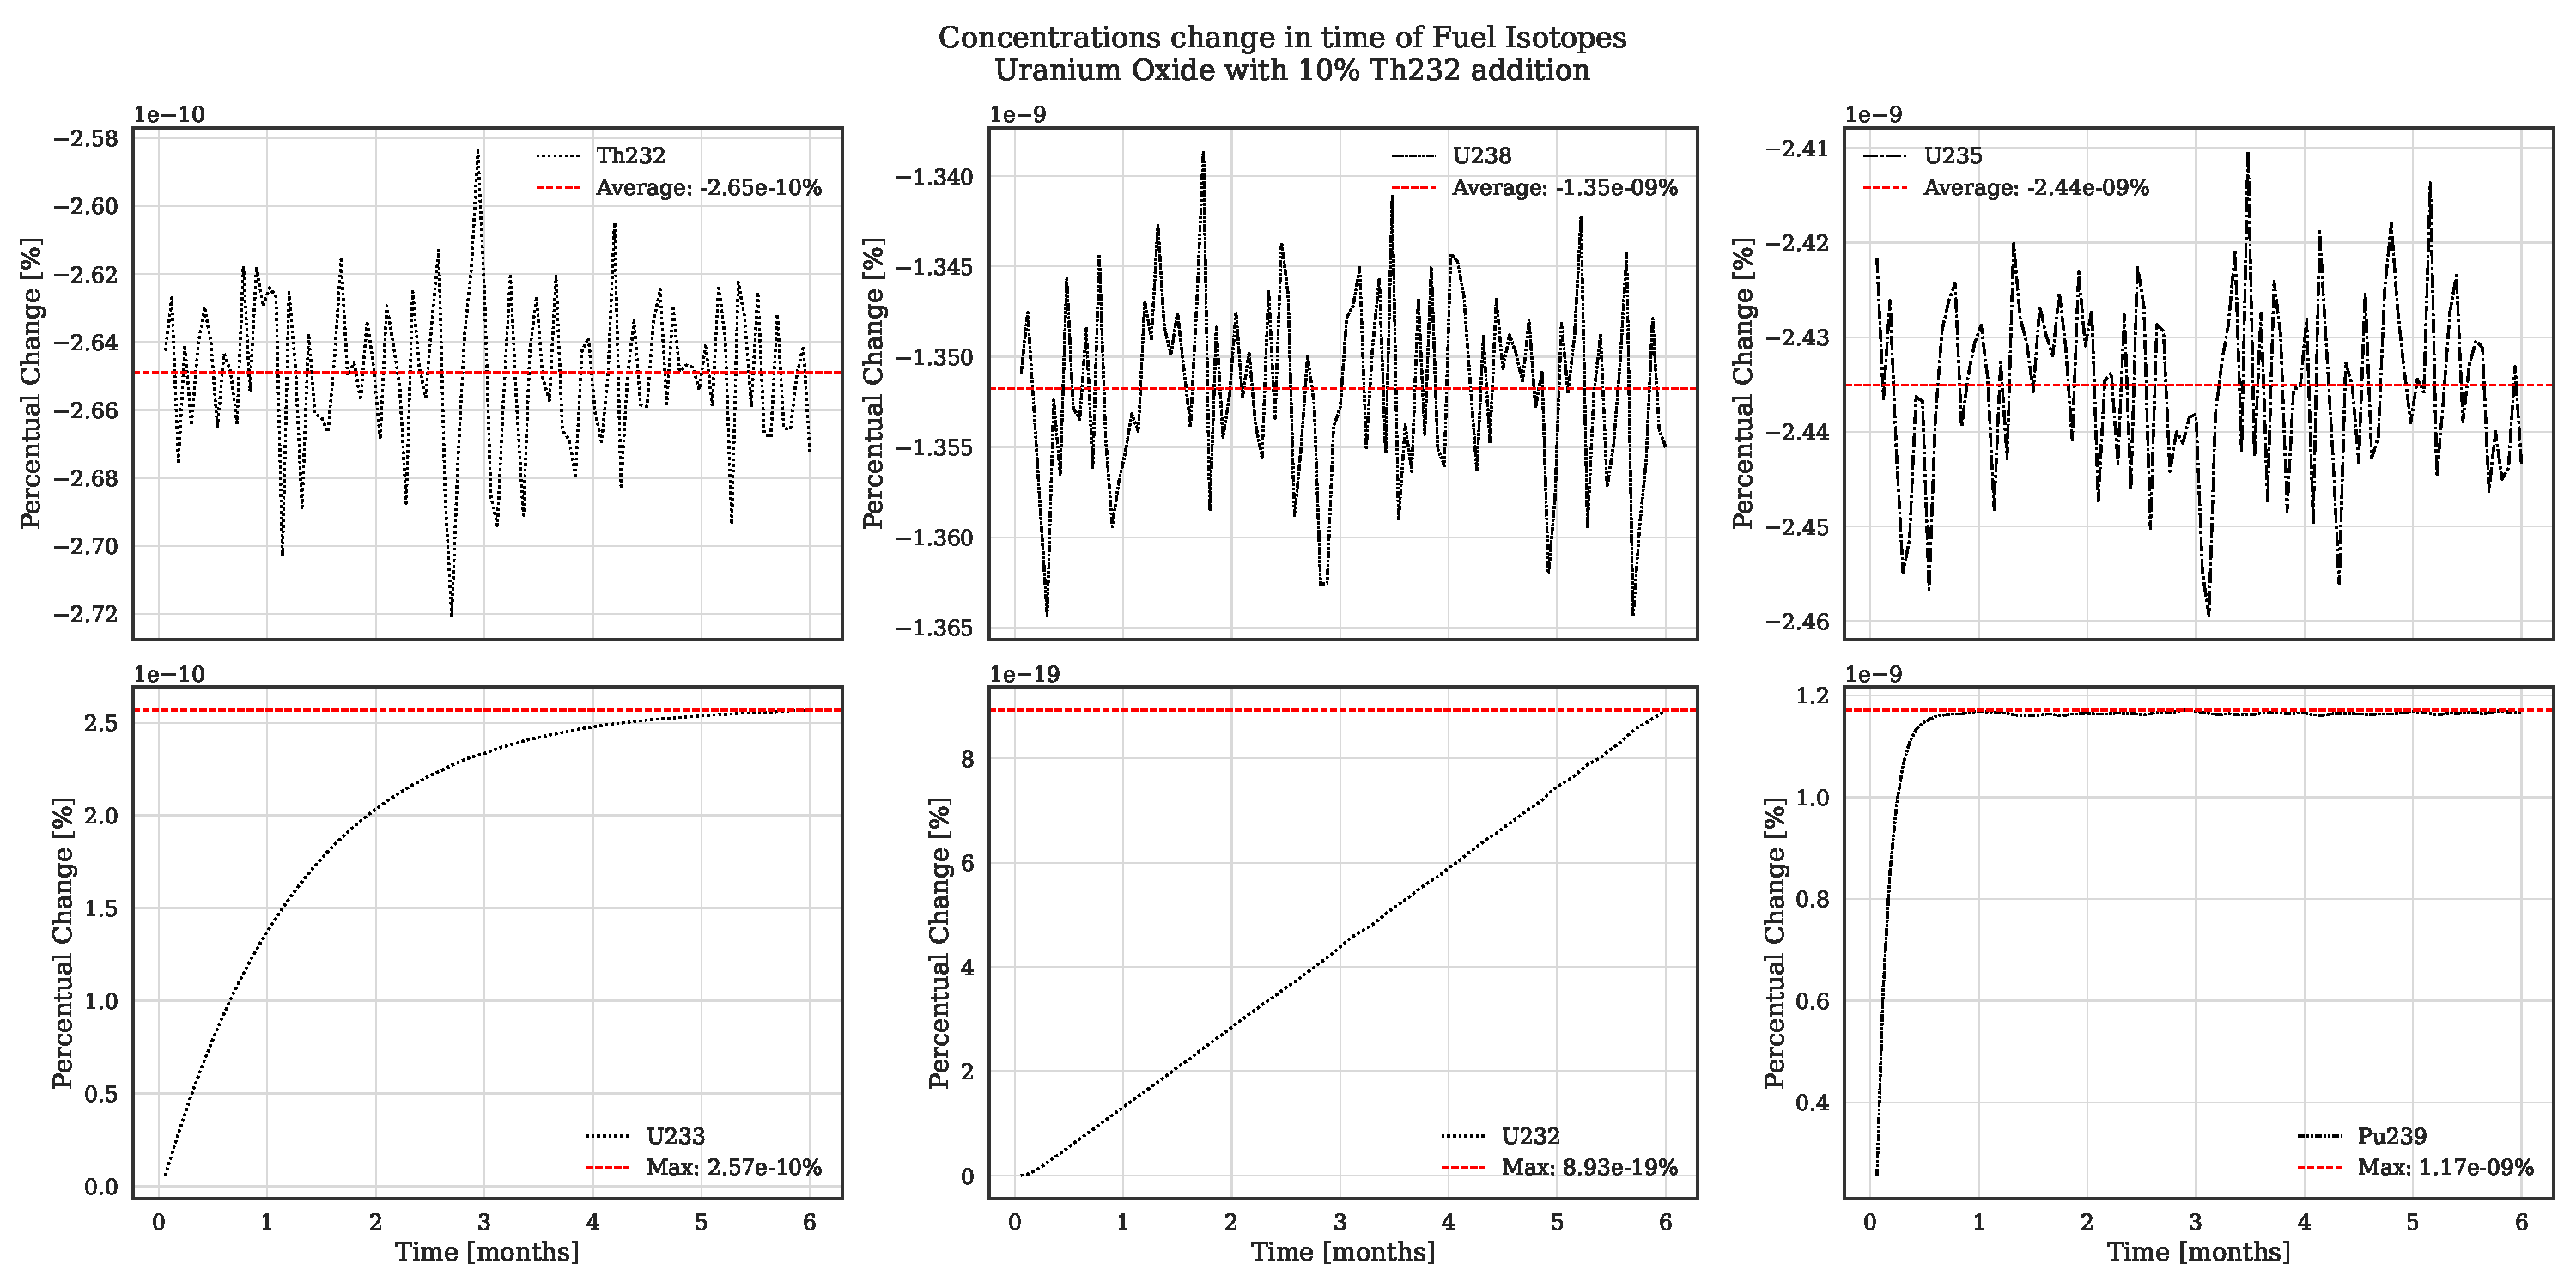
\includegraphics[scale=0.25]{percentual_change_th232_con_10.pdf}
    \captionof{figure}{\footnotesize Isotopes concentration in the fuel as function time for a \(10\%\) thorium concentration.}
    \label{fig:Th_10}
  \end{center}

  \begin{center}
    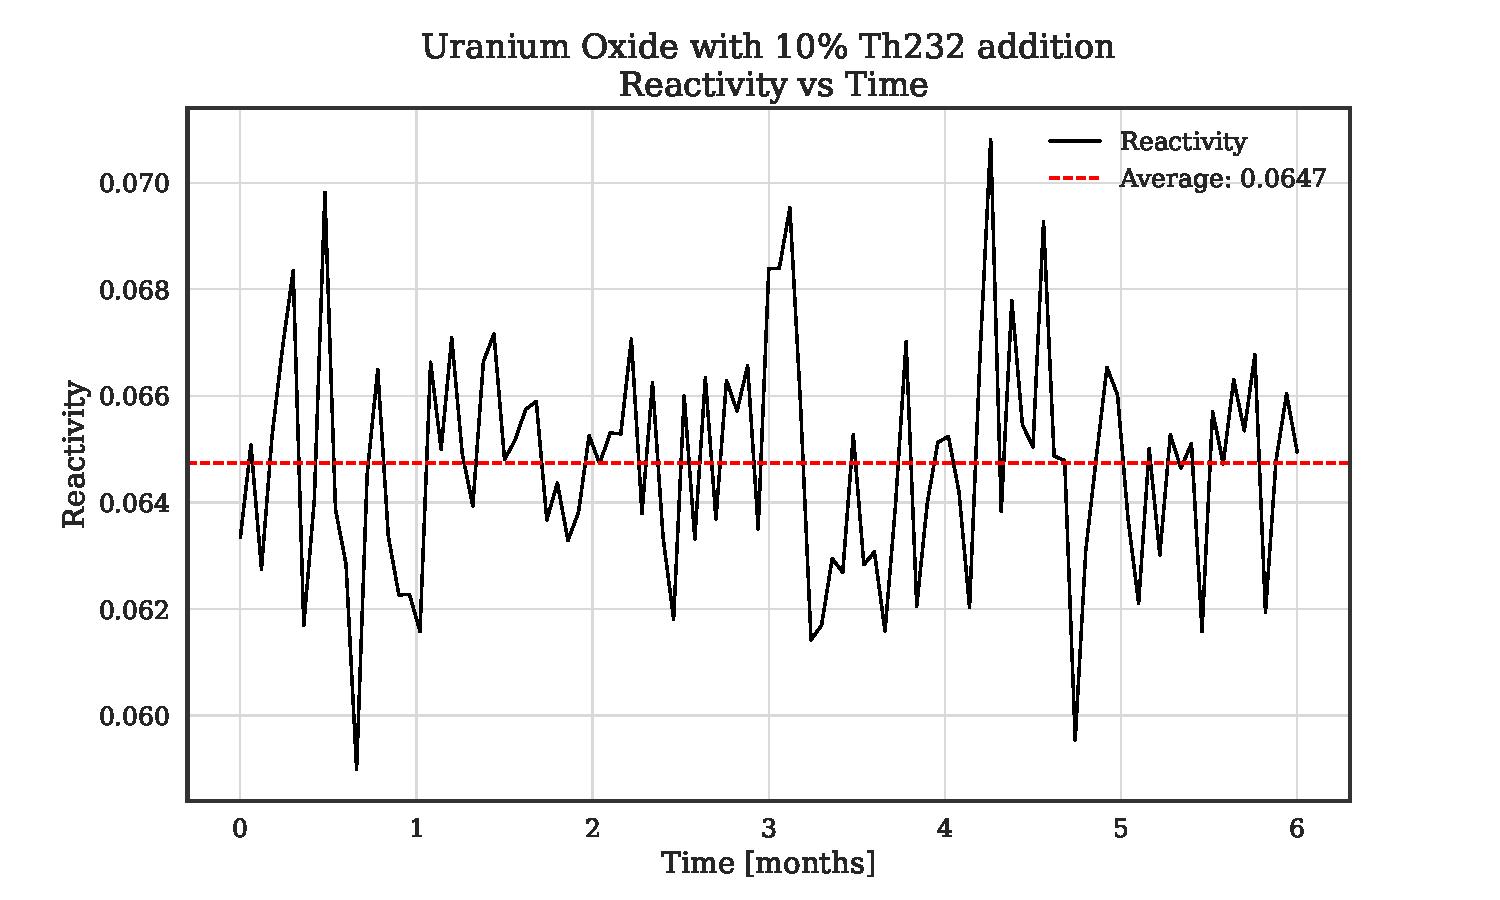
\includegraphics[scale=0.3]{Reactivity_vs_Time_UOX_10.pdf}
    \captionof{figure}{\footnotesize Reactivity as function of time.}
    \label{fig:Th_10_r}
  \end{center}


  Additional simulations explored thorium-based fuel with thorium oxide and \(10\%\) plutonium as the seed isotope. Results demonstrate that the fuel assembly achieves a critical state and attains a breeding ratio for the production of \(\prescript{233}{}{U}\), showcasing the potential for sustainable fuel generation. 

}

\headerbox{4. Conclusions}{name=Conclusions, column=1,below=Results, span=2}{ 
  The study demonstrates that thorium-based fuels, particularly ThOX with plutonium, can achieve breeding but exhibit higher reactivity, necessitating optimized fuel composition and core configurations. Thorium, as a fertile material, cannot sustain a chain reaction independently and requires external support for activation. Despite its potential benefits, the implementation of thorium fuel cycles faces significant challenges, including historical political inaction and current economic hurdles in reprocessing irradiated thorium fuel. These factors have hindered its widespread adoption in modern reactors. Further research and development are essential to overcome these challenges and fully realize the potential of thorium as a sustainable nuclear fuel.
}

\headerbox{ References}{name=References, column=0,below=Simulations,span=1}{

\scriptsize
\renewcommand{\section}[2]{\vskip 0.05em} % Get rid of the default "References" section title
%\nocite{*} % Insert publications even if they are not cited in the poster

\bibliographystyle{naturemag}
\bibliography{poster} % Use sample.bib as the bibliography file
}

\end{poster}

\end{document}